\documentclass{article}
\usepackage{nips15submit_e,times}
\usepackage{hyperref}
\usepackage{url}
\usepackage{amsmath}
\usepackage{amsfonts,amssymb}
\usepackage{graphicx}
\hypersetup{hidelinks}

\title{Weekly Report(Sep.17,2018-Sep.22,2018)}

\newcommand{\fix}{\marginpar{FIX}}
\newcommand{\new}{\marginpar{NEW}}

\begin{document}

\maketitle

\begin{abstract}
  Sorry for a long time suspension of learning. In the last week, I learned lecture1 to lecture5 of \textbf{\href{https://www.youtube.com/playlist?list=PL3FW7Lu3i5JvHM8ljYj-zLfQRF3EO8sYv}{CS231n}} and week1 of \textbf{\href{https://www.coursera.org/learn/neural-networks/home/welcome}{Neural Networks for Machine Learning}}. Because week1 is the introduction part which can be seen also in CS229, so I didn't write them in this paper.
\end{abstract}

\section{CS231n}
\subsection{Image Classification}
When we see a picture, our brain can tell us what is it. For example, when we see this image below, we say it is a cute cat. But our computer doesn't work like this. What it sees are pixels. So, if we want computer to do image classification, we need to help computer to learn classification through different pixels of different objects.
\begin{center}
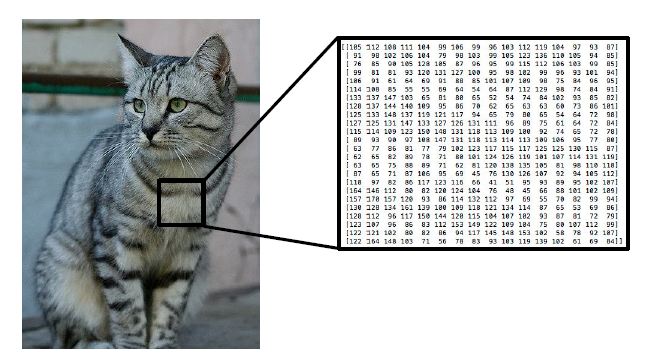
\includegraphics[scale=0.8]{cat_.png}
\end{center}
Unlike sorting a list of numbers, there are no obvious ways to hard-code the algorithm for recognizing a cat, or other classes. Thus, we seek from Data-Driven Approach:
\begin{enumerate}
  \item Collect a dataset of images and labels.
  \item Use Machine Learning to train a classifier.
  \item Evaluate the classifier on new images.
\end{enumerate}
\subsubsection{Nearest Neighbor}
We can try this simple way to do classification, which defines the nearest neighbors are of the same kind. By memorizing all data and labels, it can predict the label of the most similar training image. However, this method is not so good like what this image below shows. We can see there is a yellow part in the center of green part, and those boundaries seem like fingers, which all indicate incorrectness.
\begin{center}
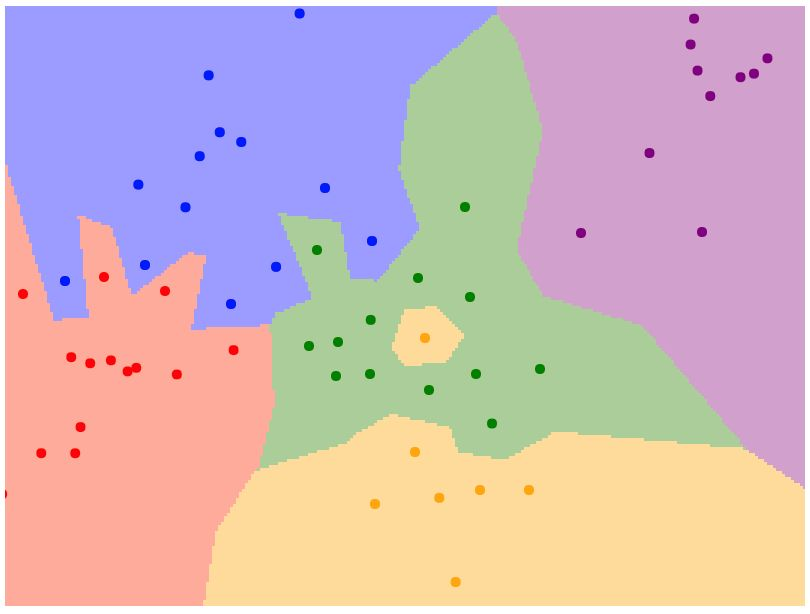
\includegraphics[scale=0.3]{neighbor.jpg}
\end{center}

\subsubsection{K-Nearest Neighbors}
Instead of copying label from nearest neighbor, take majority vote from K closest points. When K gets larger, the outcome looks better.
\begin{center}
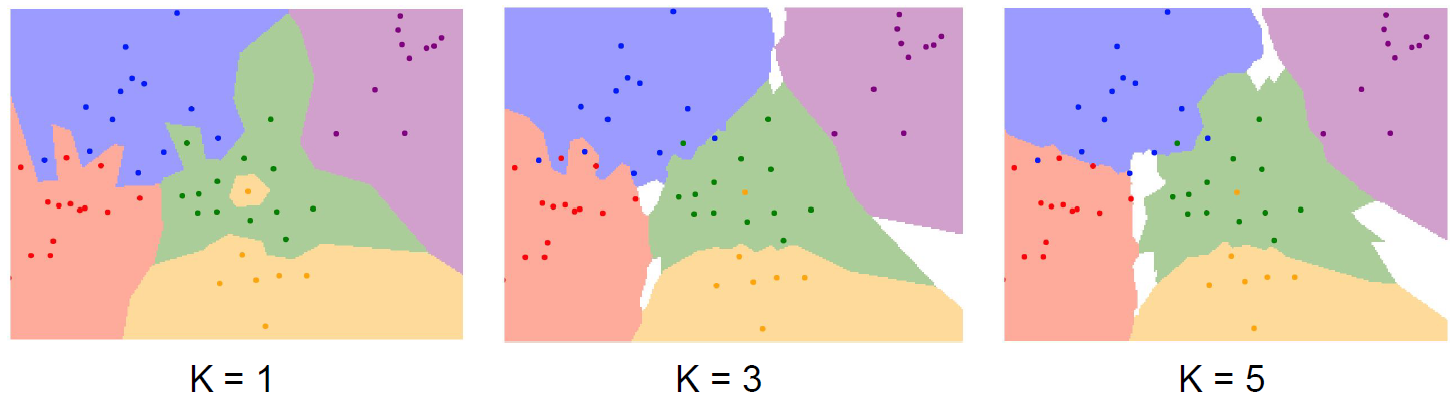
\includegraphics[scale=0.5]{K.png}
\end{center}

\subsubsection{Distance Metric}
We can measure distance by two ways. One is L1 (Manhattan) distance:
\[d_1(I_1,I_2) = \sum\limits_p|I_1^p - I_2^p|,\]
the other is L2 (Euclidean) distance:
\[d_2(I_1,I_2) = \sqrt{\sum\limits_p(I_1^p - I_2^p)^2}.\]
The picture below shows what these distance mean, the left is L1 distance and the right is L2 distance.
\begin{center}
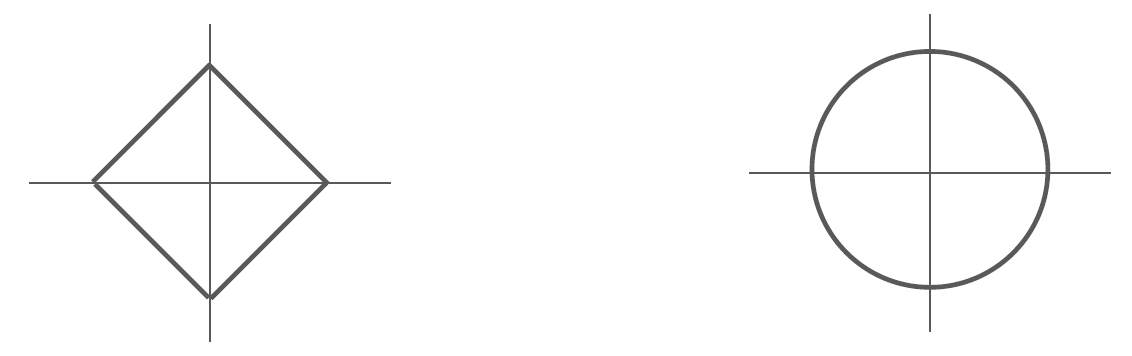
\includegraphics[scale=0.5]{distance.png}
\end{center}

\subsubsection{Setting Hyperparameters}
When we set our program, we always need to know what is the best value of k to use and what is the best distance to use. These are hyperparameters problems, that is, choices about the algorithm that we set rather than learn. Our idea is Cross-Validation: split data into folds, try each fold as validation and average the results.

But actually, k-Nearest Neighbor on images is never used. Because it is very slow at test time and distance metrics on pixels are not informative. And curse of dimensionality will result in huge amount of calculation. So, let's try parametric approach: Linear Classifier.

\subsection{Linear Classifier}
What we'll do can be illustrated like:
\[f(x,W) = Wx + b\]
\begin{center}
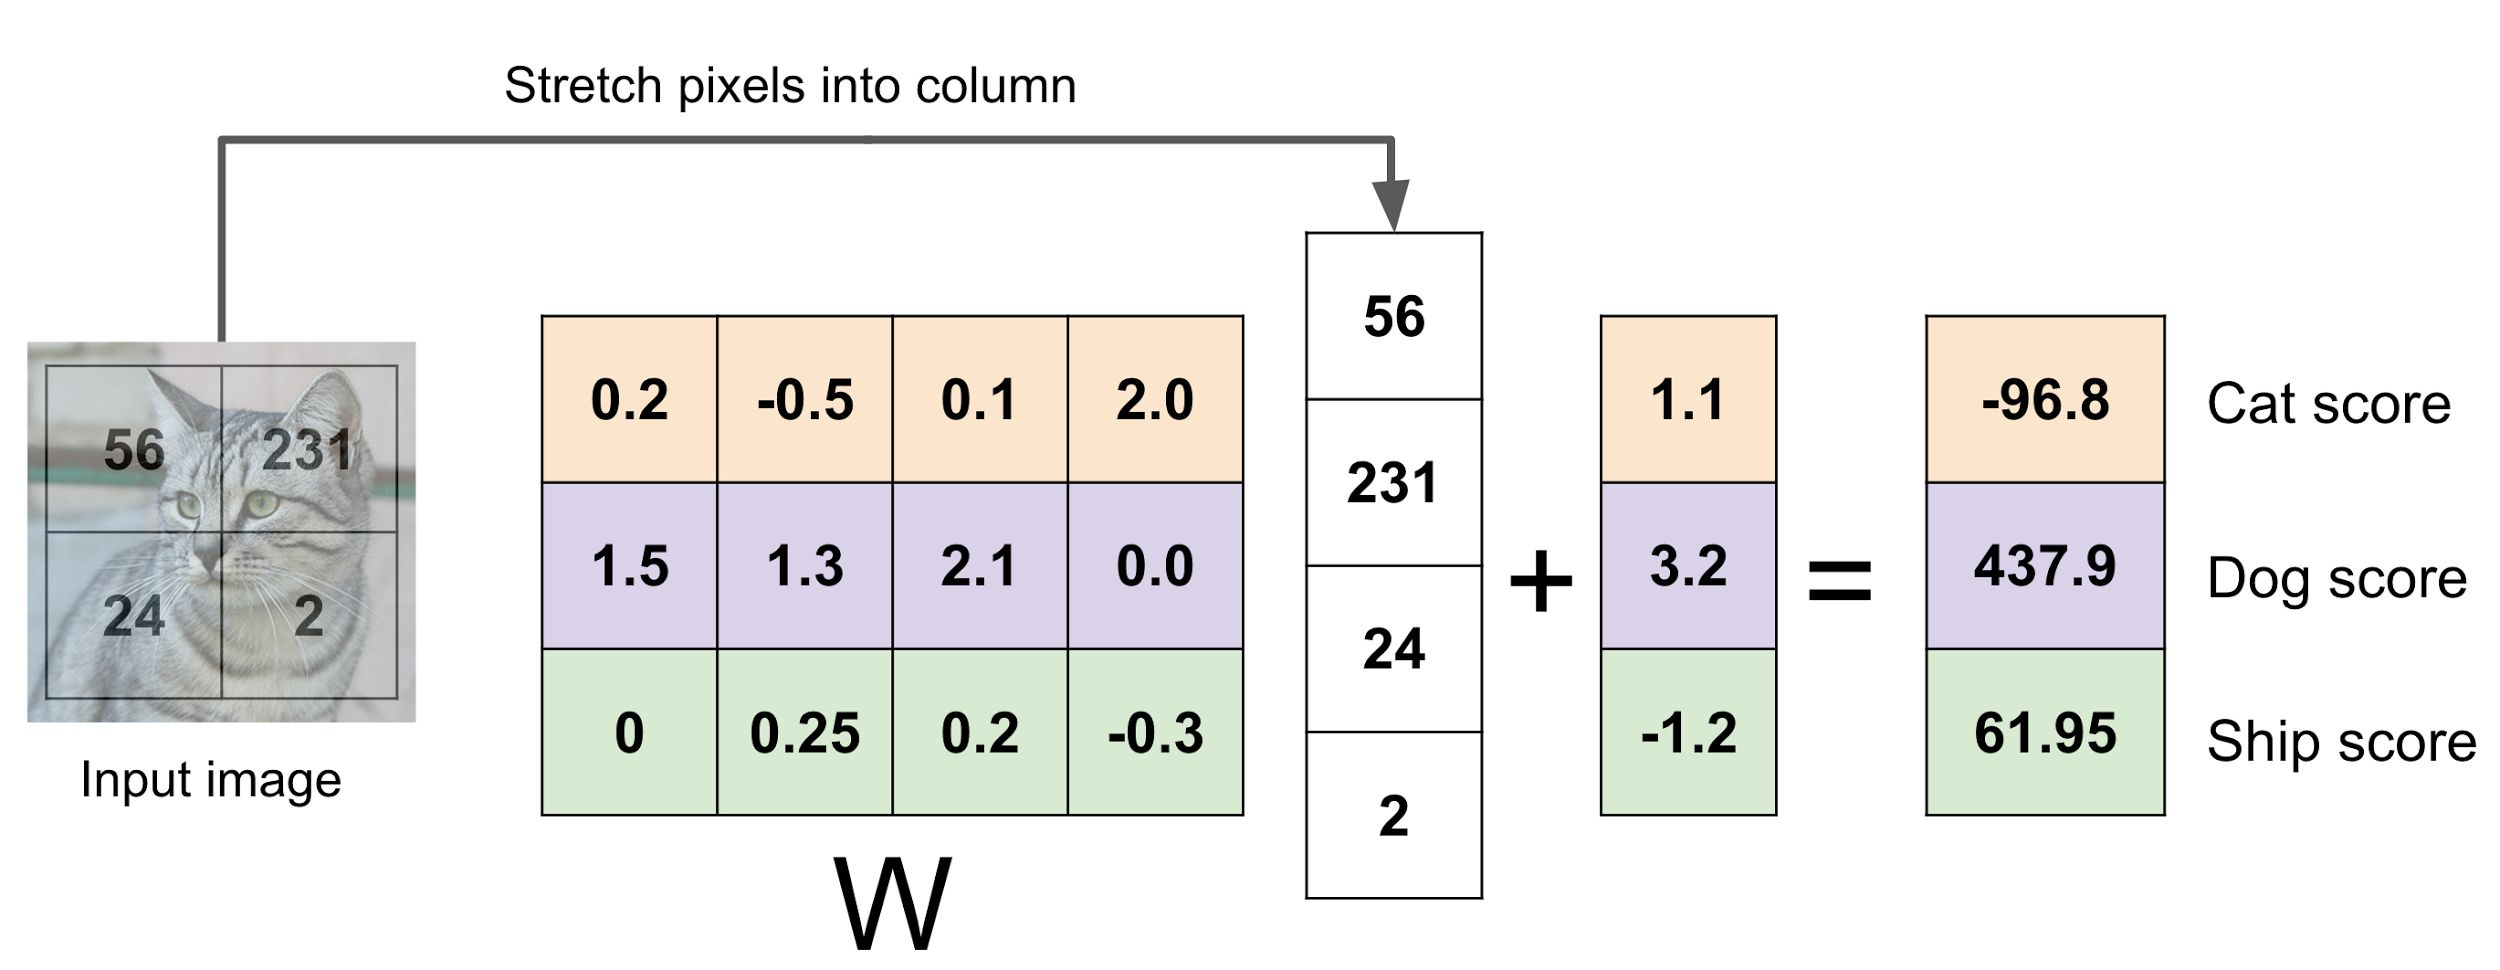
\includegraphics[scale=0.8]{linear.jpg}
\end{center}

Let's define a loss function that quantifies our unhappiness with the scores across the training data and come up with a way of efficiently finding the parameters that minimize the loss function.

\subsubsection{Multiclass SVM Loss}
\[L_i = \sum_{j\neq y_i}\max(0, s_j - s_{y_i} + 1)\]
\[L = \frac{1}{N}\sum_{i=1}^N\sum_{j\neq y_i}\max(0, f(x_i;W)_j-f(x_j;W)_{y_i} + 1)\]
Suppose that we found a $W$ such that $L = 0$. Is this $W$ unique? The answer is not. $2W$ is also has $L = 0$. But what if another $W_i$ that doesn't have linear correlation with $W$? Is there any possibility?

\subsubsection{Regularization}
But in real time we sometimes get this outcome:
\begin{center}
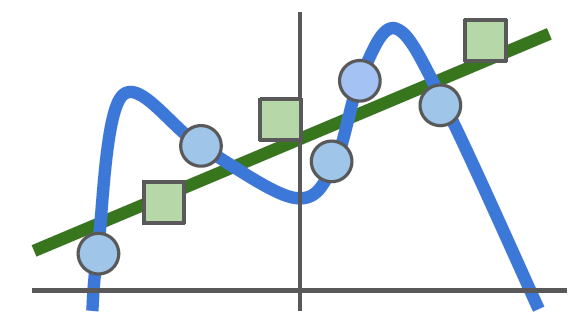
\includegraphics[scale=0.6]{regu.png}
\end{center}
We get the blue output in our training data, however, our test data may distribute like those green points. So we apply regularization to our loss function.
\[L(W) = \frac{1}{N}\sum\limits_{i=1}^N L_i(f(x_i, W), y_i) + \lambda R(W)\]

\subsection{Softmax Classifier}
The loss function of softmax classifier is
\[L_i = -\log(\frac{e^{s_{y_i}}}{\sum_j e^{s_j}})\]

\subsection{Optimization}
When we do optimization, the suggested way is always using analytic gradient and checking implementation with numerical gradient. This is called a gradient check.
\[\nabla_WL(W) = \frac{1}{N}\sum\limits_{i=1}^N\nabla_WL_i(x_i,y_i,W) + \lambda\nabla_WR(W)\]
But as there are so many data, it is impossible for us to write down every gradient. Thus, backpropagation is essential.


\subsection{Backpropagation}
Backpropagation is a method used in artificial neural networks to calculate a gradient that is needed in the calculation of the weights to be used in the network. The image below shows its process generally.
\begin{center}
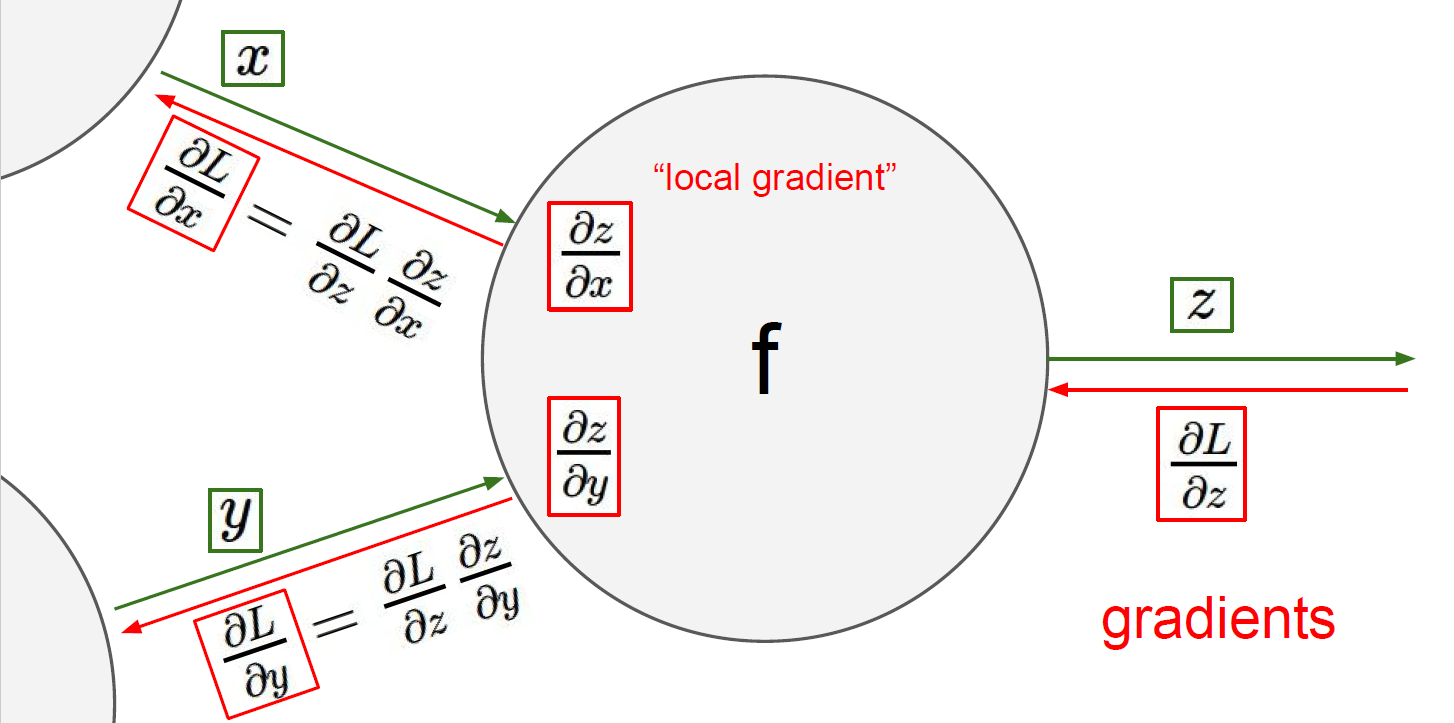
\includegraphics[scale=0.3]{back.png}
\end{center}

\subsection{Convolutional Neural Networks}
There is a long history of CNN, and scientists pay more attention to it nowadays.
\begin{center}
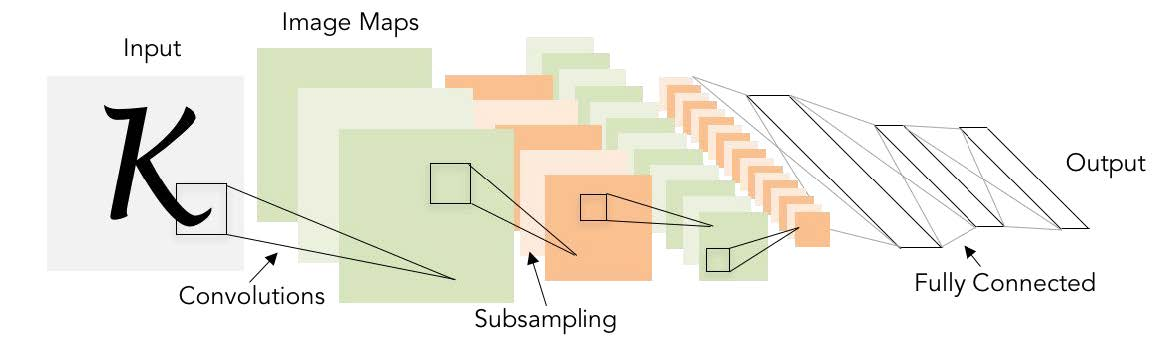
\includegraphics[scale=0.5]{cnn.jpg}
\end{center}

\subsubsection{Fully Connected Layer}
For an example, if we get a $32\times 32\times 3$ image, we can stretch it to $3072\times 1$. And 1 number is the result of taking a dot product between a row of $W$ and the input.
\begin{center}
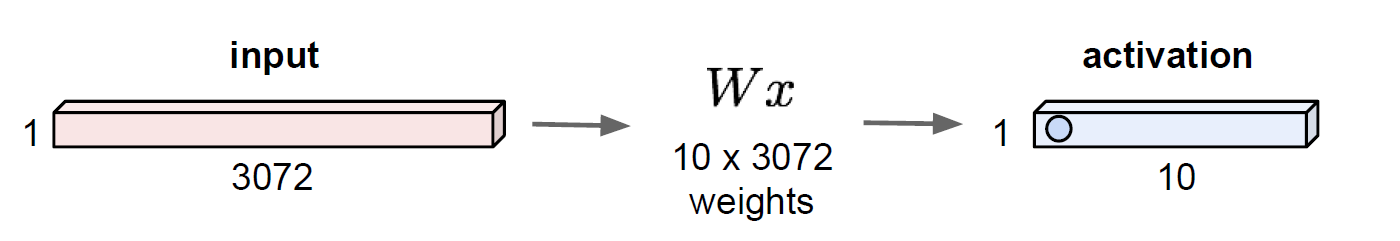
\includegraphics[scale=0.5]{layer.png}
\end{center}
But to preserve spatial structure, we use convolution layer.

\subsubsection{Convolution Layer}
Instead of stretching the image, we keep the structure. And we use a 3D filter to convolve, slide over the image spatially and compute dot products.
And the 1 number is the result of taking a dot product between the filter and a small chunk of the image. And we know the output size is equal to

(N - F) / stride + 1. To maintain the size of output, we do zero padding. But it is confusing. Doesn't it change the information of the image?

\section{Plans for Next Week}
Well, I really need to think about how to adjust my time for my major assignments are so many that I'm afraid that I'll fail them if not spent time appropriately.
\begin{enumerate}
  \item Learn lecture6 to lecture10 of  \textbf{CS231n}.
  \item Learn week2 and week3 of \textbf{Neural Networks for Machine Learning}.
\end{enumerate}

\end{document}
